% chap4_nonfactoid.tex
%

\mychapter{Improving Non-factoid Question Answering}
\label{chapter:non-factoid}

\noindent

Even though factoid questions represent a big portion of user information needs, there are many other types of questions, that do not fit into this category, \eg why-questions, how-to questions \etc
For the majority of such questions modern search engines still provide users with ``10 blue links'' only.
Extracting relevant pieces of information from search results is often quite challenging.
With the goal of improving the performance of automatic question answering systems for such generic user information needs in 2015 TREC started a series of LiveQA evaluation campaigns\footnote{http://trec-liveqa.org}.
In TREC LiveQA the task is to develop a real-time system to answer real user questions, that are posted live to Yahoo! Answers\footnote{http://answers.yahoo.com/} community question answering platform.
This chapter describes my experience participating in this shared task and research I propose to do to improve non-factoid question answering.

\section{Problem}
\label{section:non-factoid:problem}

User information needs are very diverse, which is reflected in variety of different types of questions, that people post to community question answering websites~\cite{harper2010question,ignatova2009annotating,liu2008understanding}.
Different types of questions require different type of response, which further complicates the problem of automatic question answering.
For example, procedural how-to questions are usually answered with a list of instructions, causal why-questions require a passage with certain explanations, whereas some recommendation questions could be answered with an option (\eg hotel name) and possibly some supporting statements.

Previous research on non-factoid question answering either focused on a small subset of questions (\eg definition questions~\cite{hildebrandt2004answering}), or considered this as a problem of ranking existing answers in CQA archives, which can be reused to answer new questions~\cite{carmel2000eresponder,Shtok:2012:LPA:2187836.2187939}.
The later strategy of retrieving similar previously posted questions turned out to be quite effective, as it allows a system to return a naturally looking answer in cases when a good match was found.
However, many similar questions are formulated differently, which complicates the retrieval problem, additionally many incoming information needs are still unique and there are simply no similar questions in the archive.
In this case, the system has no other option but to fall back to retrieving potentially relevant passages from regular document collections, such as the web.
The system I developed to participate in TREC LiveQA shared task combines these data sources in a single framework, which selects the answer to return from a single pool of candidate answers.
The problem of selecting best answer sentence received a lot of attention in recent years\footnote{http://aclweb.org/aclwiki/index.php?title=Question\_Answering\_(State\_of\_the\_art)}, and some of this results generalize well to selecting whole passages~\cite{diwang_lstm_2015}.
The candidate ranking module of my system builds on some of these results.
However, individual passages, and even answers to similar questions, often provide just a portion of relevant information a user might want to get.
Therefore, a problem of answer summarization becomes quite important~\cite{liu2008understanding,pande2013summarizing,tomasoni2010metadata}.
In my thesis I am planning to work on this problem and the proposed research is described later in this chapter.

In section~\ref{section:non-factoid:approach} I will describe a system I developed to participate in TREC LiveQA shared task, which establishes a baseline for future experiments.
The overview of the system was published in the proceedings of TREC 2015 conference~\cite{savenkov_liveqa15}.
Section~\ref{section:non-factoid:proposal} describes the proposed research to improve the performance of non-factoid question answering.

\section{Approach}
\label{section:non-factoid:approach}

% -=-=-=-=-=-=-=-=-=-=-=-= LiveQA : Begin -=-=-=-=-=-=-=-=-=-=-=

In this section, I describe the architecture of the automatic question answering system, which I developed to participate in TREC LiveQA shared task.
The system builds on some existing research on question answering and is based on a combination of CQA archive and web search based approaches.
There are a lot of different types of questions that users post to CQA websites and it is probably beneficial to study them separately.
However, for simplicity the model I built treats all questions in the same way.
My system is based on a single trained model, that ranks a set of extracted answer candidates and returns the top one as the response.
Preliminary analysis of questions and potential answer sources gave an insight that the best data source is answers to similar questions in case they exist and we can find them.
People often have similar tasks and situations which pose same questions.
Therefore, it is frequently the case that a similar question was already asked by someone and potentially even received a good reply and can be reused to answer new questions \cite{Shtok:2012:LPA:2187836.2187939}.
Of course, many questions or their details are unique, which makes it impossible to find a good match from the existing answers.
Therefore I also use web search to generate additional answer candidates.
For non-factoid questions it is harder to use the redundancy of the information on the web, which is exploited very effectively in factoid QA \cite{lin2007exploration}.
The system I developed extracts passages containing question terms from all retrieved web documents independently.
For training I used the publicly available collection of QnA pairs from Yahoo! Answers.
The assumption made was that for each question the answer selected as the ``best answer'' on Yahoo! Answers is indeed the best and should be ranked higher than answers to other questions.
However, taking all other answers is intractable and probably detrimental as almost all of them would be totally unrelated to the subject of the given question.
Therefore, I used search to retrieve a set of similar questions and took their answers as negative examples.
The following chapters describe the QA system in more detail.

\subsection{System architecture}
\label{section:non-factoid:liveqa:architecture}

\begin{figure}
	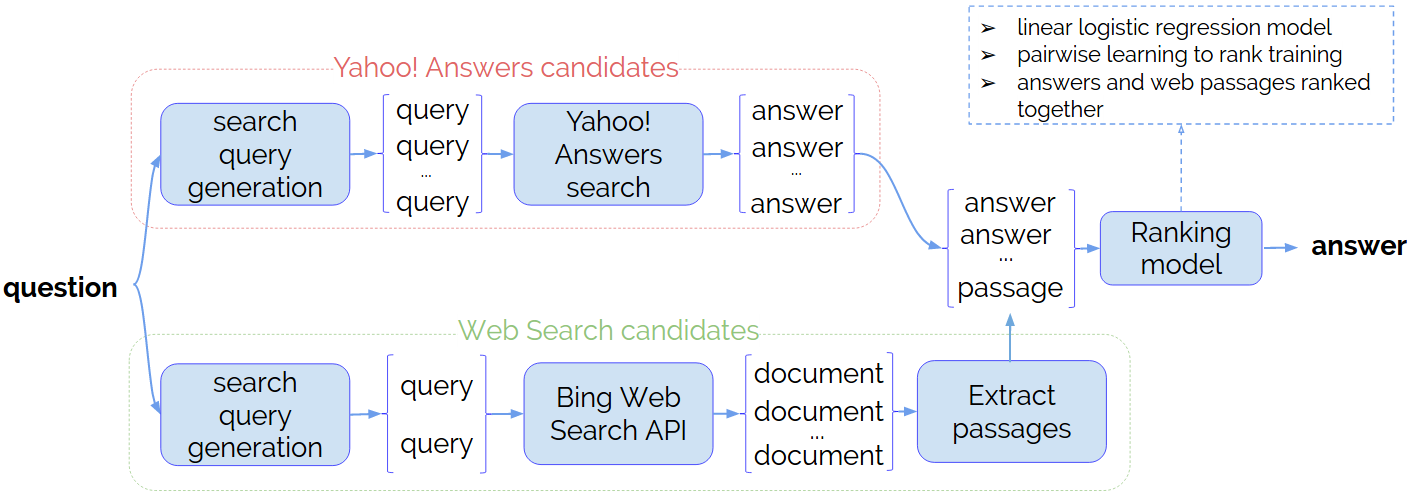
\includegraphics[width=\textwidth]{img/liveqa_qa_model}
	\caption{Architecture of the question answering system I developed to participate in TREC LiveQA shared task}
	\label{figure:non-factoid:liveqa:qa_model}
\end{figure}

The general architecture of our question answering system is presented on Figure~\ref{figure:non-factoid:liveqa:qa_model}.
It uses two primary data sources for generating answer candidates: answers to similar questions from Yahoo! Answers website and documents retrieved using web search. 
All candidates are mixed together, ranked and the top answer is returned.

\subsubsection{Candidate generation}
\label{section:non-factoid:liveqa:architecture:candidates}

Each question issued to a QA system in TREC LiveQA consists of 3 main parts: title, body and category.
For example:

\vspace{3mm}
\begin{tabular}{|p{15cm}|}
\hline
\textbf{Question category}: Astronomy \& Space\\
\textbf{Question title}: Why do people claim the Earth is not the center of the universe?\\
\textbf{Question body}: Clearly the sun and moon are moving around the Earth otherwise we would not have night and day.\\
\hline
\end{tabular}
\vspace{3mm}

When the QA system receives a question it first generates a set of candidate answers from Yahoo! Answers and regular web search.
To generate a set of candidates the system produces several search queries and issues them to both resources.

To find similar questions and extract the corresponding answers from Yahoo! Answers we use the search functionality already available on the website.
Some questions are very concise while other provide many useful as well as redundant details.
Ideally we want to match as many of them as possible, however, there is a chance that search will not return any results if there are no good matches.
Therefore the system generates a set of search queries of different granularity, issues them all to Yahoo! Answers search and collects top 10 responses from all of them.
Here is the list of queries that our system generates:
\begin{itemize}
	\item Concatenation of question title and question body (with and without stopwords)
	\item Question title only (with and without stopwords)
	\item Question title concatenated with question body and question category
	\item Question title concatenated with the name of the question category
	\item Top 5 terms from question title scored by tf-idf\footnote{Document frequency is computed on WebScope collection of QnA pairs from Yahoo! Answers}
	\item Top 5 terms from question title and body scored by tf-idf
\end{itemize}

For each query and top-10 retrieved questions the system extracts its top answer if provided and puts it into the candidate pool along with some information about the corresponding question and its category.

To extract candidate passages from relevant web documents previous research in factoid question answering have tried query reformulations \cite{Agichtein:2001:LSE:371920.371976} to better match the potential answer text.
However recently \cite{tsai2015web} demonstrated that such reformulations are no longer necessary as search engines have improved the query processing techniques.
Inspired by this observation and considering that retrieving web documents and extracting passages from them is more time consuming, the system issues only 2 web search queries: question title and title concatenated with body. 
I used Bing Web Search API\footnote{http://datamarket.azure.com/dataset/bing/searchweb} and the system downloads top-10 retrieved documents, parses HTML code and extracts the main content text \cite{Kohlschutter_2010}.
Document content is further split into sentences \cite{manning-EtAl:2014:P14-5} and candidates are built by taking contiguous sequences of sentences no longer than the answer character limit\footnote{In the final run the limit was 1000 characters}.
The model only keeps passages that contain at least one non-stopword from the question.
Web search snippets are also included as candidates.

\subsubsection{Candidate ranking}
\label{section:non-factoid:liveqa:architecture:ranking}

A trained linear logistic regression model is used to rank candidate answers, represented with a set of features:
\begin{itemize}
\item answer text statistics: length in character, tokens and sentences, average number of tokens per sentence.
\item Okapi BM25 scores, which consider question title and concatenation of title and body as queries. Term statistics were computed on Yahoo! Answers WebScope dataset. The score is calculated as follows:
\begin{equation*}
\label{equation:bm25}
\text{score}(A,Q) = \sum_{i=1}^{n} \text{IDF}(q_i) \cdot \frac{f(q_i, A) \cdot (k_1 + 1)}{f(q_i, A) + k_1 \cdot (1 - b + b \cdot \frac{|A|}{\text{avg\_al}})}
\end{equation*}
where $f(q_i, A)$ is frequency of term $q_i$ in the answer text, $k_1=1.2$, $B=0.75$ and $avg_al=50$ (average answer length).
\item term matches features: lemmas, part of speech tags of matched terms between the question and answer texts, the fraction of unique question terms matched in the answer, length of the maximum span of matched terms in the answer.
\item number of matched terms between the question title, body and the title of the page from which the candidate answer is retrieved. For Yahoo! Answers the text of the retrieved question is used as title.
\item category match feature for Yahoo! Answers candidates.
\item pairs of lemmas from question and answer texts, that are supposed to bridge the lexical gap between question and answer language.
\item average, minimum and maximum normalized pointwise mutual information (NPMI) scores between pairs of terms from the question and answer texts. The scores are estimated from QnA pairs from Yahoo! Answers WebScope dataset using the following formula:
\begin{equation*}
\begin{split}
\operatorname{npmi}(q_i;a_j) = \frac{pmi(q_i;a_j)}{-\log p(q_i,a_j)}\\
\operatorname{pmi}(q_i;a_j) = \log\frac{p(q_i,a_j)}{p(q_i)p(a_j)} =  \log\frac{p(a_j|q_i)}{p(a_j)}
\end{split}
\end{equation*}
\item QnA pair score from a Long Short Term Memory (LSTM) neural network model, described in Section~\ref{section:non-factoid:liveqa:architecture:training}.
\end{itemize}

The candidate with the highest score is returned as the answer to the question.
If something goes wrong and no candidates were generated or some problem occurred the system returns ``I do not know'' as the default answer.

\subsubsection{Model Training}
\label{section:non-factoid:liveqa:architecture:training}

There are two trained models used in the system: LSTM recurrent neural network based model, which is used as one of the features for the final logistic regression model that scores all candidates and selects the best one as the answer.
I use WebScope Yahoo! Answers dataset\footnote{https://webscope.sandbox.yahoo.com/catalog.php?datatype=l} (different splits are used) to generate training data for both LSTM and ranking model, Figure~\ref{figure:non-factoid:liveqa:model_training} describes the steps I took to build training datasets.

\begin{figure*}
	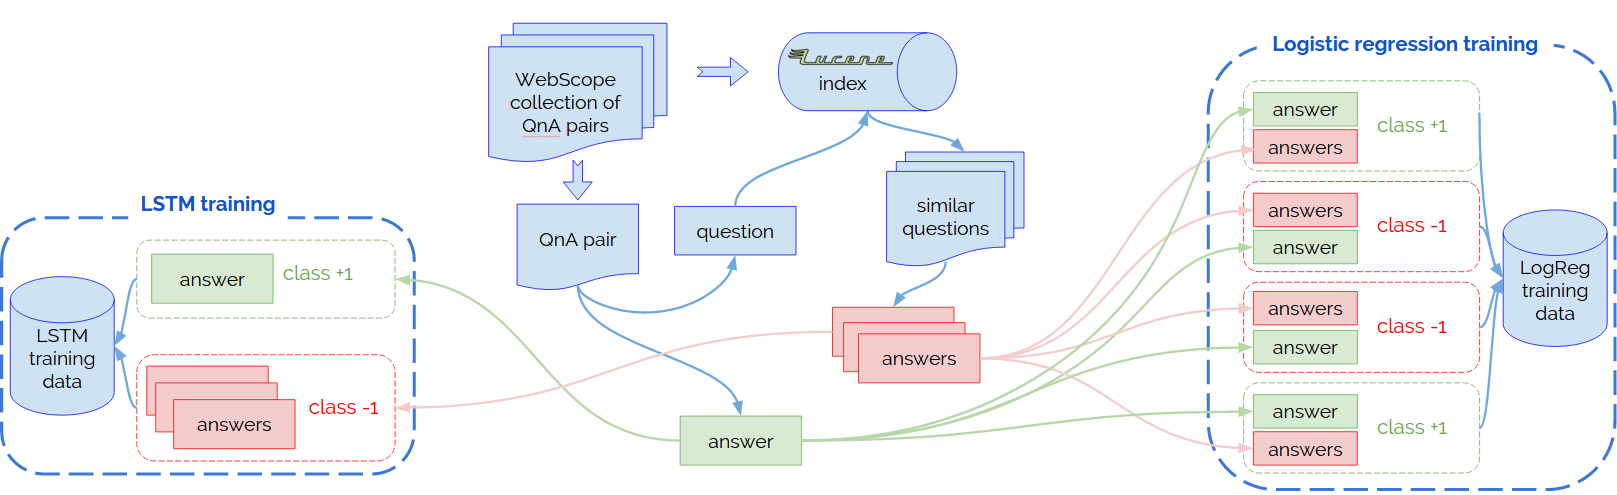
\includegraphics[width=470px]{img/liveqa_model_training}
	\caption{Workflow for generating training datasets for LSTM and answer ranking logistic regression model from the Yahoo! Answers QnA pairs}
	\label{figure:non-factoid:liveqa:model_training}
\end{figure*}

\textbf{LSTM model}.
Deep learning models had a huge success in image and speech problems and showed very promising results in natural language processing and question answering, e.g. \cite{yu2014deep,diwang_lstm_2015} to name a few.
I decided to explore this direction and built a recurrent neural network model to score how well a candidate answers a question.
Long Short-Term Memory (LSTM) \cite{hochreiter1997long} is a particular architecture of recurrent neural networks that helps with the exploding and vanishing gradients problems.
The model I developed reads question and answer tokens and produces a probability score based on a vector representation of a QnA pair.
Figure~\ref{figure:non-factoid:liveqa:lstm_model} shows the structure of the model.

\begin{figure}
	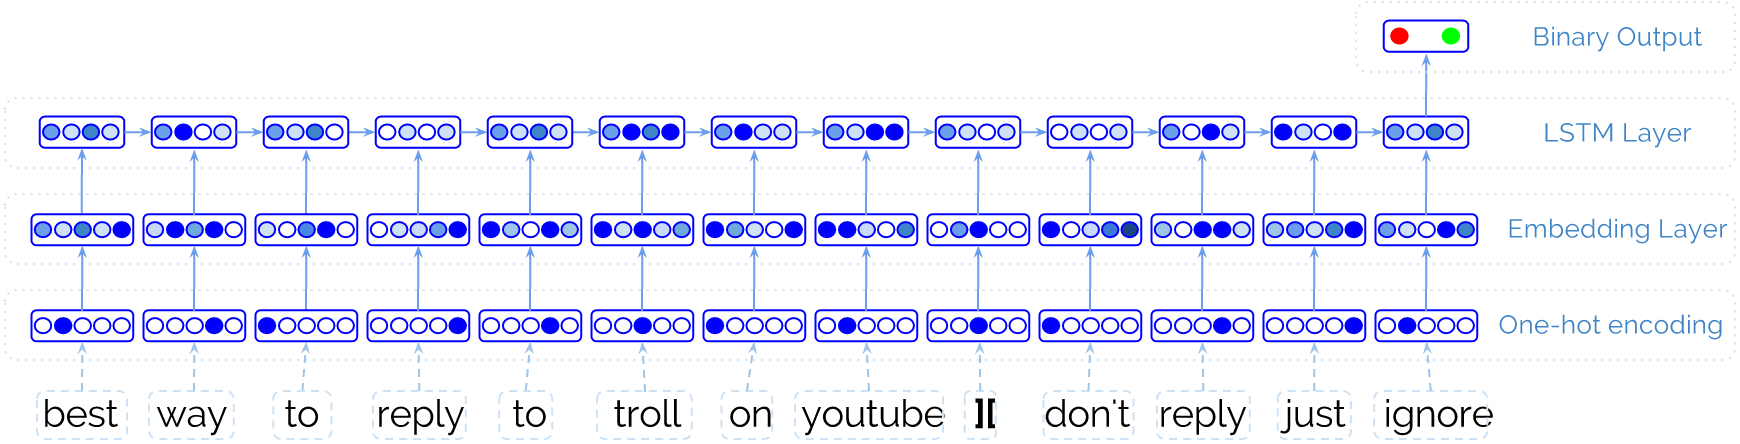
\includegraphics[width=\textwidth]{img/liveqa_qa_lstm}
	\caption{LSTM model for answer scoring. The example shows a QnA pair where the question is ``Best way to reply to trolls on youtube?'' and the answer is ``Do not reply, just ignore''.}
	\label{figure:non-factoid:liveqa:lstm_model}
\end{figure}

Question (title with body) and answer texts are tokenized, punctuation characters are removed and for each token lowercase lemma is taken.
The sequences are limited to 100 elements and concatenated through a sentinel separator character so the model could learn where the question ends and the answer starts.
The hidden state of the model after the whole sequence is processed is used by logistic regression unit to output a probability, that a candidate answers the question well.

To train the model QnA pairs from Yahoo! Answers WebScope dataset were used (we selected a subset of questions from the categories chosen for TREC LiveQA).
Each question and the corresponding best answer was used as a positive training example.
Random negative examples would be too unrelated to the current question, therefore I chose to use answers to similar questions only.
All QnA pairs were indexed with Lucene\footnote{https://lucene.apache.org/} and similar questions were retrieved using the built-in BM25 retrieval model.
For each question and correct answer pair from the dataset 10 similar questions were retrieved and the corresponding answers were used as negative examples for training\footnote{It is true, that some of them can indeed be relevant to the original question}.

The model was implemented using Keras\footnote{http://keras.io} library.
I used an embedding and hidden layers of dimension 128 and the vocabulary size of 1M words.
The model was trained using Adam optimization technique \cite{kingma2014adam} with mini batches of 200 instances for 100 epochs.

\textbf{Logistic regression model}.
The final model that ranks all answer candidates is a linear L2-regularized logistic regression model.
To train the model we used a different split of QnA pairs from Yahoo! Answers WebScope dataset.
For each question the corresponding ``best answer'' is taken as the correct one.
To get a sample of negative examples Lucene index is used again and answers to 10 most similar questions are retrieved.
Different from LSTM model training, here I took a pairwise approach for learning to rank and generated training examples from pairs of different answers to the same question, where one answer is the correct one.
That is, let the current question be $Q$, its ``correct'' answer $A^*$, and retrieved candidates $A_1, ..., A_n$.
Each candidate is represented with a set of features: $f(Q, A^*)$, $f(Q, A_1)$, ..., $f(Q, A_n)$.
For each $i=1..n$ we create two training instances, i.e. class 1: $\langle A^*, A_i\rangle$ and class -1: $\langle A_i, A^*\rangle$.
Each such instance is represented with pairwise differences of features, e.g. $\langle A^*, A_i\rangle: f_{pair}(Q, \langle A^*, A_i\rangle) = f(Q, A^*) - f(Q, A_i)$.
The trained model is linear, therefore if $w(f(Q, A^*) - f(Q, A_i)) > 0$ then $w f(Q, A^*) > w f(Q, A_i)$ and we can rank candidates by the score produced by the model, i.e. $w f(Q, A_i)$.

\subsection{Evaluation}
\label{section:non-factoid:liveqa:evaluation}

From the final run of the system, 1087 questions were judged by the organizers on a scale from 1 to 4:\\
\textbf{4: Excellent} - a significant amount of useful information, fully answers the question\\
\textbf{3: Good} - partially answers the question\\
\textbf{2: Fair} - marginally useful information\\
\textbf{1: Bad} - contains no useful information for the question\\
\textbf{-2} - the answer is unreadable (only 15 answers from all runs were judged as unreadable).

The following performance metrics were reported:

\begin{itemize}
\item \textbf{avg-score(0-3)}: average score over all questions, where scores are translated to 0-3 range. This metric considers ``Bad'', unreadable answers and unanswered questions, as scored 0.
\item \textbf{s@i+}: the fraction of answers with score i or greater (i=1..4)
\item \textbf{p@i+}: the number of questions with score i or greater (i=2..4) divided by the number of answered questions
\end{itemize}

Table \ref{table:liveqa-results} provides the results of top 5 teams by average answer score, results for our system and average scores.
Please refer to the \cite{overviewliveqa15} for more details and results of all systems.

\begin{table}
	\centering
	\begin{tabular}{|p{3cm}|p{2cm}|p{1.3cm}|p{1.3cm}|p{1.3cm}|p{1.3cm}|p{1cm}|p{1cm}|p{1cm}|}
		\hline
		& \# answers & avg score (0-3) & s@2+ & s@3+ & s@4+ & p@2+ &  p@3+ & p@4+ \\
		\hline
		1. CMUOAQA & 1064 & 1.081 & 0.532 & 0.359 & 0.190 & 0.543 & 0.367 & 0.179 \\
		2. ecnucs & 994 & 0.677 & 0.367 & 0.224 & 0.086 & 0.401 & 0.245 & 0.094\\
		3. NUDTMDP1 & 1041 & 0.670 & 0.353 & 0.210 & 0.107 & 0.369 & 0.219 & 0.111\\
		4. RMIT0 & 1074 & 0.666 & 0.364 & 0.220 & 0.082 & 0.369 & 0.223 & 0.083\\
		5. Yahoo-Exp1 & 647 & 0.626 & 0.320 & 0.211 & 0.095 & 0.538 & 0.354 & 0.159\\
		\hline
		7. Emory & 884$\downarrow$ & 0.608$\uparrow$ & 0.332$\uparrow$ & 0.190$\uparrow$ & 0.086$\uparrow$ & 0.408$\uparrow$ & 0.233$\uparrow$ & 0.106$\uparrow$\\
		\hline
		Average results & 1007 & 0.467 & 0.262 & 0.146 & 0.060 & 0.284 & 0.159 & 0.065\\
		\hline
	\end{tabular}
\caption{Results of the TREC LiveQA evaluation of Emory University QA system and average results of all systems. $\uparrow$ means that results of Emory system in this metric are above average, and $\downarrow$ means that results are below average}
\label{table:liveqa-results}
\end{table}

The metric s@1+ shows the fraction of questions for which a readable answer was returned by the system.
A lower score in this metic means that my system did not return an answer in time in almost 20 \% of the cases.
A part of the problem is caused by several technical issues, that appeared on the day of the evaluation run.
Due to one of them LSTM model did not provide any score for a significant fraction of submitted questions, and the other problem made the whole system unresponsive for a couple of hours.

The absolute values of the performance metrics demonstrate a great room for improvement as our system was able to return partial or good answer only in 23\% of the cases (p@3+) when the answer was returned.
And for 60\% of the questions the answer does not contain any useful information.

\subsection{Analysis}
\label{section:non-factoid:liveqa:analysis}

\begin{figure}
	\centering
	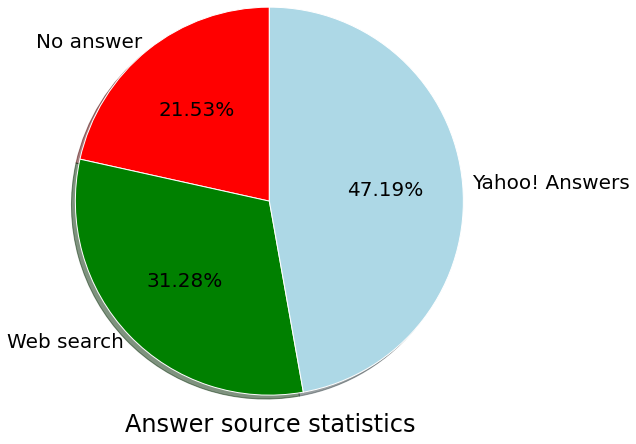
\includegraphics[width=0.5\textwidth]{img/liveqa_answer_source}
	\caption{Distribution of sources for answers returned by our system}
	\label{figure:non-factoid:liveqa:answer_source_pie}
\end{figure}

In this section we will answer some of the questions about the performance of different system components and their relative importance.

The first question, that we are going to study is the relative effectiveness of web passages and answers to previously posted questions for answering new questions.
As Figure~\ref{figure:non-factoid:liveqa:answer_source_pie} shows, almost half of all answers returned by my system were generated from Yahoo! Answers.
In $\sim$21\% of the cases our system did not return any results\footnote{This happened mainly due to a couple of technical issues that made our system unresponsive for quite some time}, and in the rest $\sim$31\% of the cases a passage from a web page was returned as the answer.
I further looked into the domains of the web pages used to generate the answer and noticed, that many more were extracted from other community question answering websites and forums.

The quality of answers generated from passages built from web search results are lower on average compared to Yahoo! Answers candidates.
Figure~\ref{figure:non-factoid:liveqa:answer_source} shows the distribution of scores for each of our data sources.
Some categories were harder than the other \cite{overviewliveqa15} and as we see on Figure~\ref{figure:non-factoid:liveqa:answer_source:category} in some cases web passages were actually more effective than answers to previously posted questions.

\begin{figure}
	\centering
	\begin{subfigure}[b]{0.38\textwidth}
		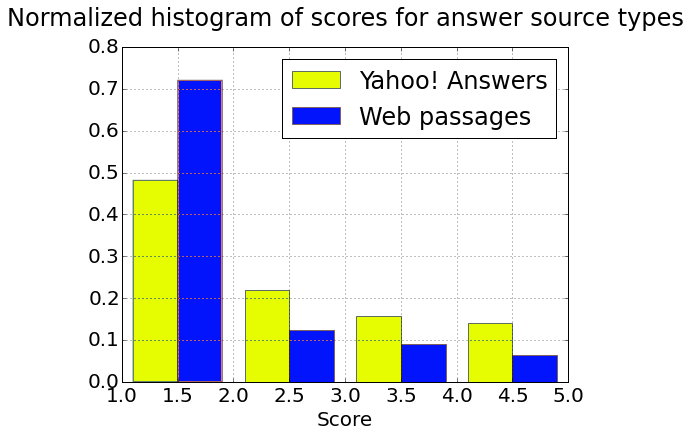
\includegraphics[width=\textwidth]{img/liveqa_answer_source_scores}
		\caption{Histogram of qrel scores}
		\label{figure:non-factoid:liveqa:answer_source:scores}
	\end{subfigure}
	\begin{subfigure}[b]{0.6\textwidth}
		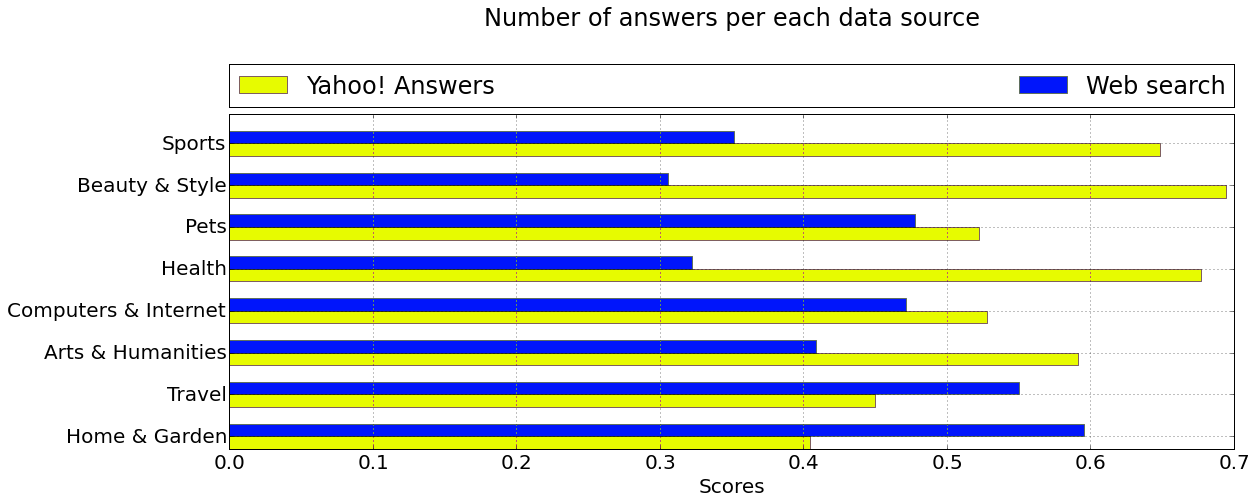
\includegraphics[width=\textwidth]{img/liveqa_answer_source_by_category}
		\caption{Average scores of answers from Yahoo! Answers and web passages for different categories}
		\label{figure:non-factoid:liveqa:answer_source:category}
	\end{subfigure}
	\caption{Comparison of web passages and Yahoo! Answers as candidate sources}
	\label{figure:non-factoid:liveqa:answer_source}
\end{figure}

\begin{figure}
	\centering
	\begin{subfigure}[b]{0.49\textwidth}
		\centering
		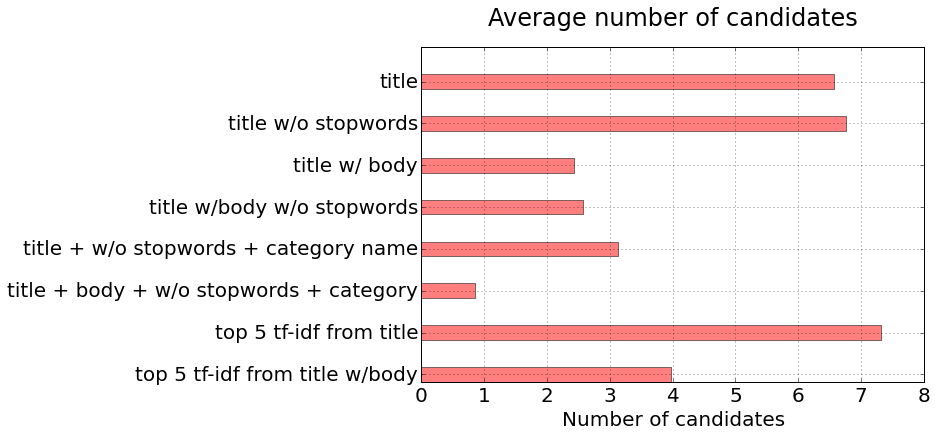
\includegraphics[width=\textwidth]{img/liveqa_query_candidate_count}
		\caption{Average number of candidates}
		\label{figure:non-factoid:liveqa:analysis:query_generation:count}
	\end{subfigure}
	\begin{subfigure}[b]{0.49\textwidth}
		\centering
		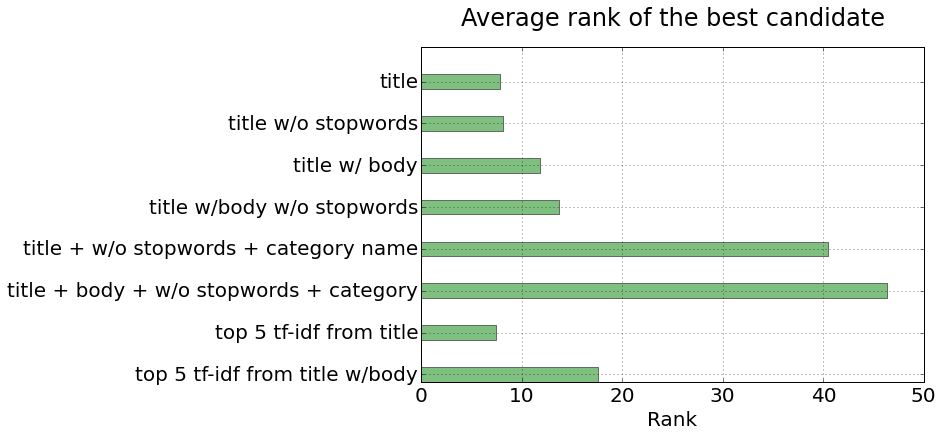
\includegraphics[width=\textwidth]{img/liveqa_query_candidate_bestrank}
		\caption{Average rank (according to our ranking model) of the best candidate}
		\label{figure:non-factoid:liveqa:analysis:query_generation:rank}
	\end{subfigure}
	\caption{Comparison of different query generation strategies for Yahoo! Answers similar questions search}
	\label{figure:non-factoid:liveqa:analysis:query_generation}
\end{figure}

The next question, that we analyze is the effectiveness of search query generation strategies.
Figure~\ref{figure:non-factoid:liveqa:analysis:query_generation} plots average number of candidates and the position of the best candidate retrieved by each of the question generation strategies.
The longer the search query the less results it retrieved, which is expected, and the lower the quality of the candidates.
As a result, in half of the cases the answer returned by our system was retrieved using just top 5 highest IDF terms as the query\footnote{The same candidate is often also retrieved by other queries}.
For web search we only used 2 query generation strategies, namely question title and concatenation of title with body.
Analogously, concatenation of title with body query had lower quality and more often returned few or no results.

Figure~\ref{figure:non-factoid:liveqa:features} demonstrates a plot of importances of different features in our answer ranking linear logistic regression model.
The feature with the highest weight is category match, but we should note, that this feature is overfitted to the way we build training set (category of the correct answer always matched the category of the question).
The next most useful feature is the cosine similarity between the page title (or question text for Yahoo! Answers) and the current question, followed by BM25 score, number of matched verbs, etc.

\begin{figure}
	\centering
	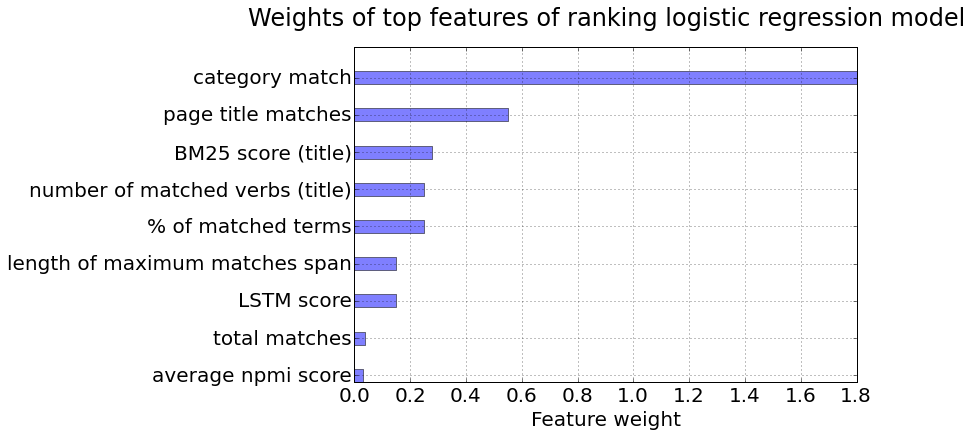
\includegraphics[width=0.6\textwidth]{img/liveqa_features}
	\caption{Weights of features in answer ranking logistic regression model}
	\label{figure:non-factoid:liveqa:features}
\end{figure}

I also looked through a small sample of our answers manually.
There are a number of typical problems, and one of them is the lack of good question semantic similarity measure.
E.g. the question \textit{``Is there a section fro the subject of writing''} in the \texttt{Books \& Authors} category retrieved a question \textit{``I ca not write in the To: Cc: Subject: section''} from the \texttt{Yahoo Mail} category.
Even though the questions have many terms in common, they are obviously semantically unrelated.
Therefore, in future we need to focus more on better question similarity measures.

Answer does not have to have many words in common with the question.
On the contrary, the maximum possible term overlap will be if a candidate is just a copy of the answer.
This was one of the problems for answers, retrieved from the web search results.
The way we used to generate the training data did not include such ``artificial'' cases, however, they are pretty common in practice.
For example, in a number of cases the answer our system chose came from a forum post and instead of selecting the answer posts, the system ranked the question post higher as it had more term matches.
The winning CMU team addressed this issue by considering answer-clue pairs, where the clue is supposed to match the question text and the former answers the question.
We plan to explore a similar strategy.

\subsection{Further improvements for TREC LiveQA 2016}
\label{section:non-factoid:liveqa:improvements}

TREC LiveQA 2016 task was run on May 31, and I made a few improvements to my system.
One of the major quality loss in my previous system was due to random crashes, which resulted in no response for more than 200 questions.
This year I changed the architecture of the system to make it more reliable and make sure the answer is returned in time.

Next, as analysis of the previous year track has revealed, many of answers generated using regular web search still came from different community question answering websites.
However, the system did not treat such pages differently from regular documents and did not extract additional meta-data, such as the question text, \etc.
Therefore, for LiveQA 2016 I decided to extend a set of data sources and in addition to Yahoo! Answers I added separate candidate generation pipelines for Answers.com and WikiHow.com.
For these verticals the system uses the search engine built into the platforms, and extracts answers along with the corresponding question meta-data.

The other improvements target the candidate answer ranking module of the system.
I've extended a set of features representing each candidate answer to include the following:
\begin{itemize}
	\item Percentage of the terms in the answer, that are not matched against the question. This features aim at estimating the new information in the answer. The previous system often selected answer that simply repeated the question.
	\item N-gram matches features: fraction of 1,2-3-grams from the question title, body that overlaps the n-grams from the answer text
	\item All term match features were computed for related question and body. More specifically, additionally to taking the answer text itself, we added features that compute similarity scores between the current question and retrieved question (title and body). For candidates, generated from regular web documents we tool the title of the page as question title, and the previous paragraph in text as body.
\end{itemize}

Additionally, I replaced the logistic regression ranking model with LambdaMART~\cite{burges2010ranknet}, as implemented in RankLib library\footnote{https://people.cs.umass.edu/$\sim$vdang/ranklib.html}.
Unlike the previous year, when training data in a usual sense did not exist, in 2016 we had relevance judgments from previous campaign.
To train the LambdaMART model I took this data and scraped the original web pages to get meta-information and generate all the features for the candidates.
Using this data I trained the model to optimize NDCG metric.
The results of the evaluation are not available at the moment.

\subsection{Summary}
\label{section:non-factoid:liveqa:summary}

The pilot year of TREC LiveQA establishes a very good baseline for the future of non-factoid question answering.
It confirmed that the task itself is quite challenging as only $\sim$35\% of the questions returned by the winning system had a score of 3 or higher, and there is still a big gap between in the quality of human and machine answers.
It will be exciting to see the next version of the task next year, and how the participants will build on this year approaches.


% -=-=-=-=-=-=-=-=-=-=-=-= LiveQA : End -=-=-=-=-=-=-=-=-=-=-=-=-

\section{Proposed Research}
\label{section:non-factoid:proposal}

The results of TREC LiveQA 2015 established a baseline performance of automatic non-factoid question answering systems, and shed some light on typical problems and future research directions.
One particular problem, that I am proposing to concentrate research in my thesis, is that passages a QA system extract as candidate answers often either contain redundant information, or, on contrary, the answer is split across multiple passages and a single one is not going to satisfy user information needs.
One way to tackle these problems is to introduce an answer summarization module, which instead of returning the top ranked answer, will generate the response by summarizing the relevant pieces of information from ranked candidates.
Existing research on answer summarization usually targets community generated answers on CQA websites, which is different from summarizing automatically generated candidates.
The developed algorithms typically follow an extractive summarization approach, and explore different answer sentences ranking strategies to either shorten the answer, cover multi-intent questions or to improve diversity~\cite{chan2012community,zhaochun_sparsecoding_2016}, and less attention is paid to the overall quality and readability of summarized answer text.

For my thesis I propose to capitalize on the recent successes of deep learning for natural language processing and apply some of the techniques on the new problem of answer summarization.
Section~\ref{section:non-factoid:proposal:method} describes the proposed methodology in more details.

\subsection{Method}
\label{section:non-factoid:proposal:method}

Distributed representations for words~\cite{mikolov2013distributed,pennington2014glove} and longer phrases~\cite{le2014distributed,kiros2015skip} opened up a new era in natural language processing and information retrieval.
Using distributed representations or embeddings one can simply calculate the similarity between words or sentences using various distance metrics in the embeddings space.
Such representations made it possible to train end-to-end models for various NLP tasks, which reach or outperform existing state-of-the-art models~\cite{collobert2011natural}.

Text summarization is not an exception, and recently a number of different architectures were proposed for both more traditional extractive~\cite{kaageback2014extractive} as well as abstractive summarization~\cite{rush-chopra-weston:2015:EMNLP,chopraabstractive16}.
In answer summarization we are dealing with multiple different piece of text, therefore it is more related to the problem of multi-document summarization~\cite{cao2015ranking}.
However, unlike document summarization, here we have a notion of the question and some answer candidates (if not the majority) might be totally irrelevant to the question and not worth including overall.

\begin{figure}
	\centering
	\begin{subfigure}{0.8\textwidth}
		\centering
		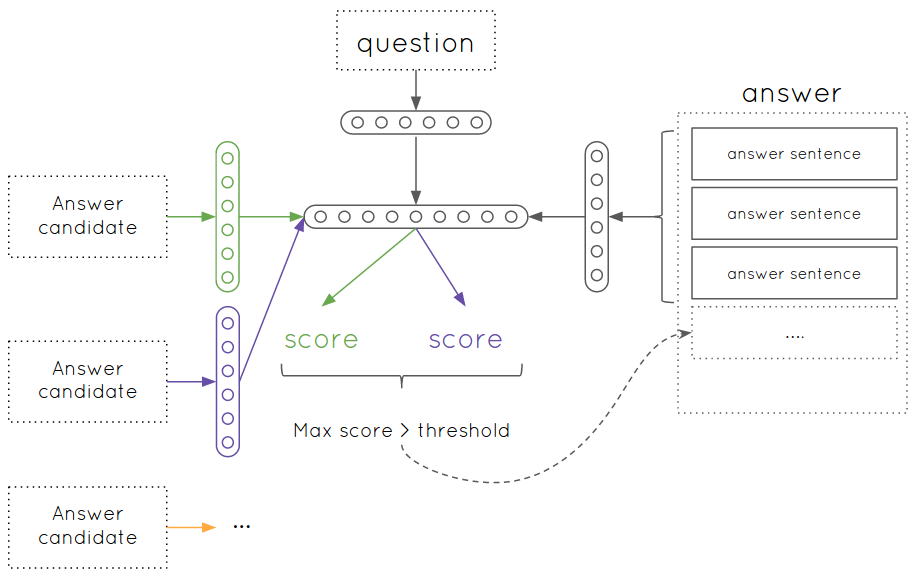
\includegraphics[width=\textwidth]{img/answer_summarization_model}
		\caption{Extractive summarization}
		\label{figure:non-factoid:proposal:model:extractive}
	\end{subfigure}
	
	\begin{subfigure}{0.8\textwidth}
		\centering
		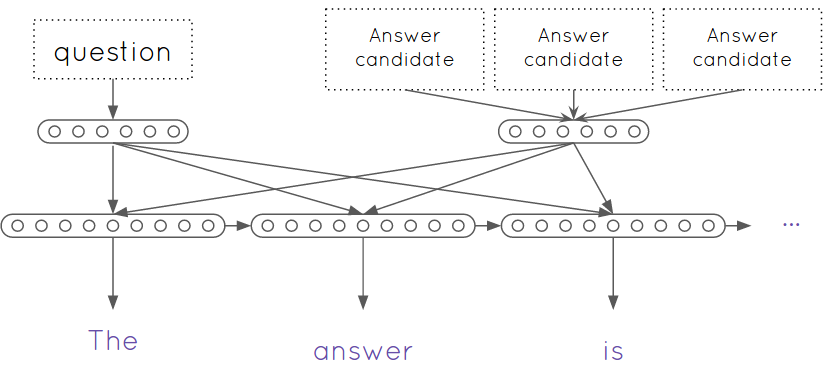
\includegraphics[width=\textwidth]{img/answer_summarization_model_abstractive}
		\caption{Abstractive summarization}
		\label{figure:non-factoid:proposal:model:abstractive}
	\end{subfigure}
	\caption{The architecture of the proposed answer summarization models}
	\label{figure:non-factoid:proposal:model}
\end{figure}

The schematic of the models I propose to implement for answer summarization is depicted on Figure~\ref{figure:non-factoid:proposal:model}.

On each step of the extractive summarization the model takes 3 kinds of inputs: embedding of the question, already constructed summary and answer candidate.
Embeddings of the question and already constructed summaries can be obtained using the attention mechanism~\cite{xu2015show} to focus the model on specific parts of the input.
The idea of abstractive summarization model is based on the sequence to sequence attention-based models, and similar in architecture to the works of Sumit Chopra and Alexander Rush~\cite{chopraabstractive16,rush-chopra-weston:2015:EMNLP}.

\subsection{Experimentation}
\label{section:non-factoid:proposal:experiments}

Since the problem of answer summarization is not new, there are some datasets already available and several benchmark results exists.
For my experiments I am planning to use the datasets of M.Tomasoni and M.Huang~\cite{tomasoni2010metadata}, which was constructed based on Yahoo! Answers archive and manually generated gold summaries, and of Adi Omari et al~\cite{omari2016novelty}, constructed for the task of novelty-based answer reranking.
In the later dataset human annotators extracted nuggets of different aspects for the same question, and therefore its possible to judge the relevance of each of the answer with respect to these nuggets.
These datasets will be used to test my extractive summarization model.
The results on the first dataset could be directly compared to other existing answer summarization techniques, \eg \cite{zhaochun_sparsecoding_2016,erkan2004lexrank,tomasoni2010metadata}.
Thus, this experiment will show if the deep learning based answer summarization model can compete with other approaches as it does for regular document summarization.
The later dataset was developed for the task of novelty-based answer ranking, \ie arranging answers in such a way that a user is exposed to different aspects and opinions.
On this dataset I will test if sentence-based answer summarization is better (in terms of diversity of covered aspects) than ranking answers under certain maximum character length limit, \ie whether extracting sentences to form an N char length summary gives a better experience than ranking complete answers under the same limit.

However, in these datasets the answer candidates were taken from community generated answers to each question, and therefore on average they are relevant.
To test the model on more realistic scenario of automatic question answering, I am planning to reuse the candidate answers with relevance labels from TREC LiveQA datasets.
I will conduct two experiments: 
\begin{itemize}
\item use the extractive summarization model trained on the previously mentioned datasets to summarize answer candidates
\item train extractive and abstractive answer summarization model using community generated answers without human labeling.
\end{itemize}

The first experiment will help me answer the question if summarizing automatically generated candidates is more difficult than community answers, and whether a model trained for one task can be used for another.
The later experiment will test the hypothesis that community generated answer can be used as a ground truth for model training, which would allow one to get millions of examples from CQA archives.
The quality of summaries will be judged manually using crowdsourcing for relevance, coherence and readability.

\section{Summary}
\label{section:non-factoid:summary}

This chapter focus on the problem of improving the performance of non-factoid question answering system.
The system I developed participated in both TREC LiveQA 2015 and 2016 shared tasks, which allowed me to test certain ideas and discover directions for future improvements.
The thesis will focus on the problem of answer summarization, and proposed extractive and abstractive summarization models, based on recent developments in the field of neural networks.

However, no matter how well an automatic system performs, there will be cases, when it is unable to generate a good response to a user question.
In such cases, computers can ask for help, which would lead to a hybrid human-computer question answering systems.
Chapter~\ref{chapter:crowdsourcing} focuses on the idea of crowdsourcing for real-time question answering.